% !TeX root = ../main-paper.tex
\section{Results}

\subsection{OCR evaluation}

\begin{figure}

\subcaptionbox{}[.5\linewidth]{
\begin{tabular}{rll}
\toprule
          & CER & CER$_{norm.}$ \\
\midrule
Pero      & 3.78\% & 3.76\% \\   
Tesseract & 6.56\% & 6.45\% \\
Kraken    & 15.72\% & 15.46\% \\  
\bottomrule
\end{tabular}

\bigskip

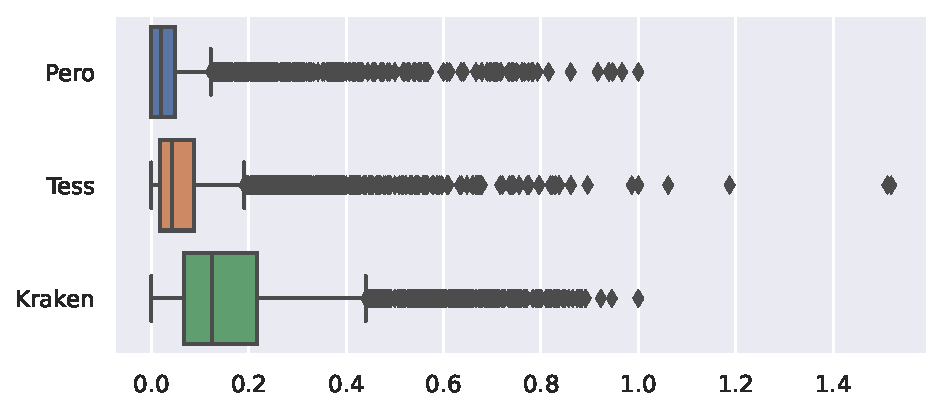
\includegraphics[width=\linewidth]{images/ocr-eval-2.pdf}
}
\subcaptionbox{}[.5\linewidth]{
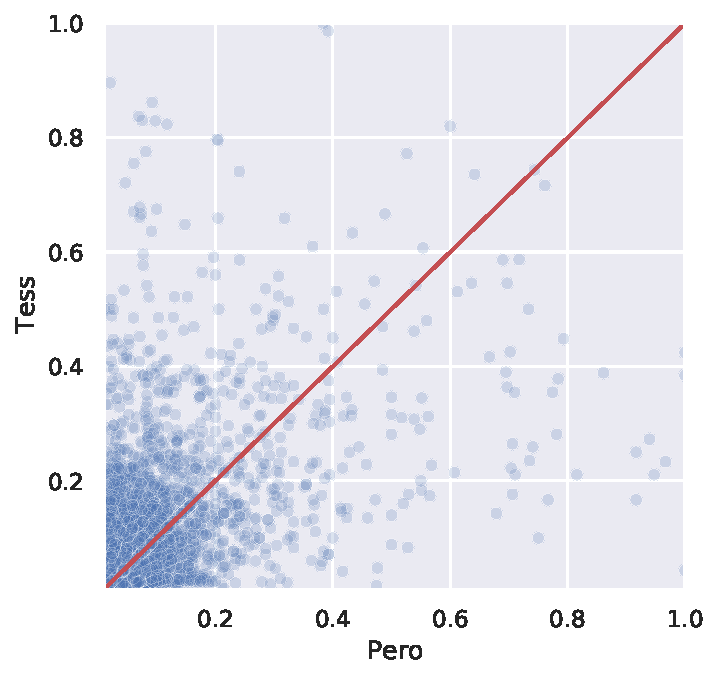
\includegraphics[width=\linewidth]{images/ocr-eval-1.pdf}
}
\caption{Character error rates at entry-level for Pero OCR and Tesseract. (a) Global CER and distribution of the CER per entry. (b):
joint plot of the dataset showing that the two systems do not fail on the same entries.}  
\end{figure}

\subsection{Experiment 1: NER sensibility to the number of training examples}
Table \ref{tab:experiment-1-models-performances} and Figure \ref{fig:f1-vs-trainsize} show the mean F1 score, precision, and recall computed on the test dataset, for 5 fine tunings of each model and for each of the 8 training subsets.
CmBERT, CmBERT+ptrn and SpaCy NER display the same behaviour: performances increase dramatically with the number of training examples and rapidly reach an area of slower progress around 1000 examples.
The F1 score increases by 4.6 points between 49 and 796 examples for CmBERT (resp. 1.6 for CmBERT+ptrn and 5.1 for SpaCy NER) but only by 1 point between 796 and 6373 examples (resp. 0.6 and 1.4).
The models derived from CamemBERT always outperform the Spacy model.

It appears that pretraining the CamemBERT model on OCRed texts seems worth it only when a the training set used to fine-tune the NER layer is small.
This effect might be due to the differences in nature between the training subsets, whose texts are manually corrected, and the noisy OCR texts used to pretrain CamemBERT.
Indeed, the learned embeddings from the pretraining are specialized on noisy texts and therefore less adapted to clean texts.
The pretraining aims at adapting the model to the vocabulary of the domain and to the errors caused by the OCR, which reveals not helpful and even counter-productive when the texts do not contain these types of errors.


\begin{table}[h!]
\centering
\caption{F1 score, precision and recall measured on the fine-tuned models CmBERT, CmBERT+ptrn and SpaCy NER in experiment 1 for 8 training sets of increasing sizes.}
\begin{tabular}{llrrrrrrrr}
       & Training examples &  49   &  99   &  199  &  398  &  796  &  1593 &  3186 &  6373 \\
       & \% & 0.8   & 1.6   & 3.1   & 6.2   & 12.5  & 25.0  & 50.0  & 100.0 \\
\midrule\bottomrule
\multirow{3}{*}{\rotatebox{90}{F1 score}} & CmBERT &  89.5 &  90.5 &  92.7 &  93.3 &  \textbf{94.1} &  \textbf{94.9} &  \textbf{94.6} &  \textbf{95.1} \\
       & CmBERT-ptrn &  \textbf{92.2} &  \textbf{92.9} &  \textbf{93.6} &  \textbf{93.8} &  93.8 &  94.1 &  \textbf{94.6} &  94.4 \\
       & SpaCy NER &  87.0 &  89.0 &  90.3 &  91.9 &  92.1 &  92.8 &  93.2 &  93.5 \\
\cline{1-10}
\multirow{3}{*}{\rotatebox{90}{Precision}} & CmBERT &  87.4 &  88.7 &  91.5 &  92.7 &  93.3 &  94.9 &  93.9 &  95.1 \\
       & CmBERT-ptrn &  90.8 &  91.8 &  92.9 &  93.0 &  93.0 &  93.4 &  94.1 &  93.9 \\
       & SpaCy NER &  85.6 &  87.7 &  90.0 &  92.0 &  92.4 &  92.8 &  93.1 &  93.7 \\
\cline{1-10}
\multirow{3}{*}{\rotatebox{90}{Recall}} & CmBERT &  91.6 &  92.5 &  93.9 &  93.9 &  94.9 &  94.9 &  95.4 &  95.1 \\
       & CmBERT-ptrn &  93.6 &  94.0 &  94.4 &  94.6 &  94.6 &  94.8 &  95.0 &  94.9 \\
       & SpaCy NER &  88.6 &  90.4 &  90.7 &  91.7 &  91.9 &  92.8 &  93.3 &  93.4 \\
\end{tabular}
\label{tab:experiment-1-models-performances}
\end{table}


\begin{figure}[h!]
	   \center{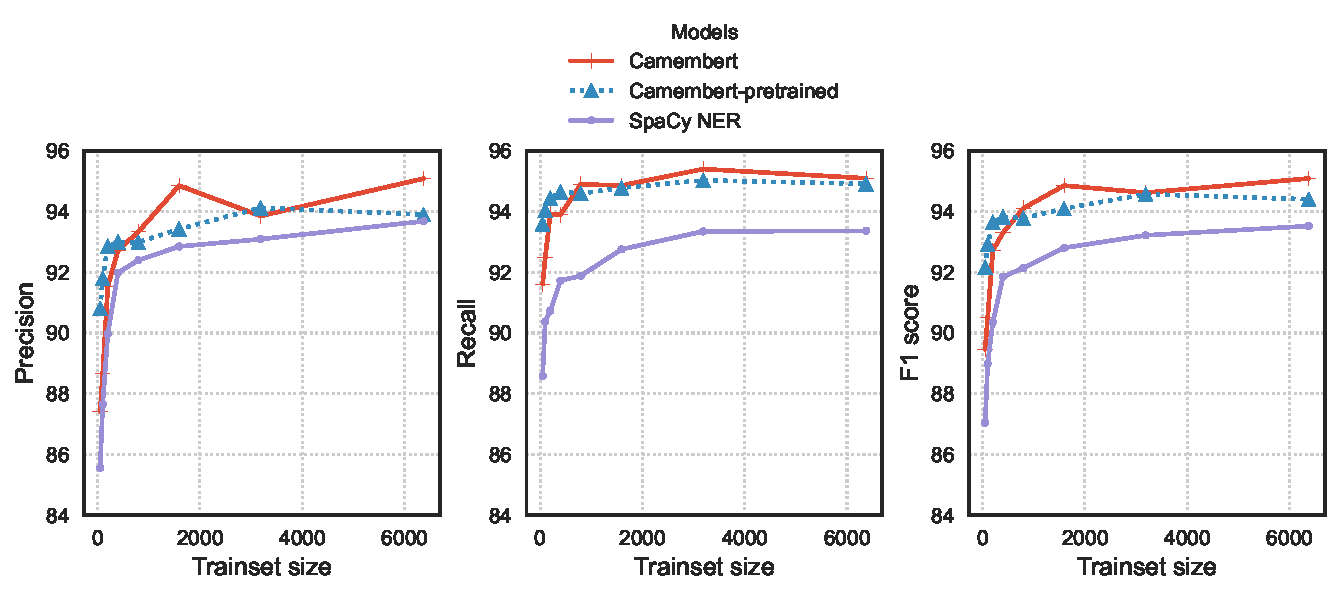
\includegraphics[width=\textwidth]
	       {images/experiment-1-models-performances.pdf}}
	  \caption{\label{fig:f1-vs-trainsize} Precision, recall and f1 score from table~\ref{tab:experiment-1-models-performances}}.
\end{figure}
	                                        


\subsection{Experiment 2: NER in the presence of noisy OCRed texts}
CmBERT and CmBERT+ptrn are fine-tuned on the training sets from reference-gold (manually corrected entries) and pero-gold to produce 4 different models.
Their F1 score measured against the test tests from reference-gold, pero-gold and tesseract-gold are given in \cref{fig:exp_2_eval_ner}.
The results clearly show that models perform best when both the pre-training and the NER fine-tuning share the same characteristics (here, OCR noise) as the texts to be processed.

In our tests, pre-training the model brings a slight gain in performance ($\approx 0.5\%$).
We did not pre-train or fine-tune with texts extracted with Tesseract.
However, despite a loss of performance the model pre-trained and fine-tuned with pero-gold still gives the best results.
This is probably due to the fact that the texts produced by Pero-OCR feature characteristics intermediary between human transcriptions and Tesseract.

\begin{figure}
    \centering
    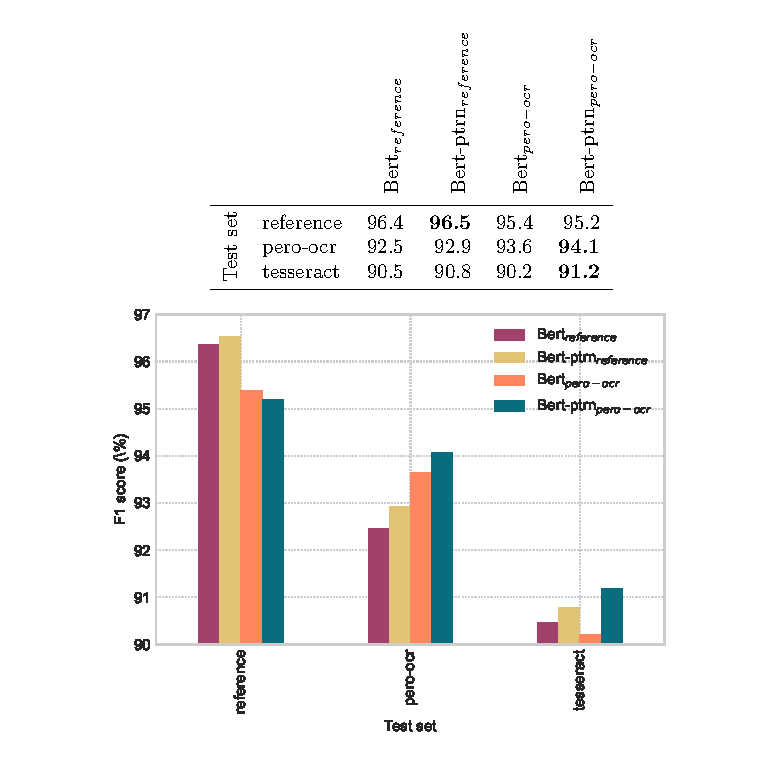
\includegraphics[width=\textwidth]{figs/eval-ner-exp2.pdf}
    \caption{F1 scores (in \%) of NER predictions in presence of OCR noise in the training and testing examples, either manually corrected or raw from Pero-OCR and Tesseract. The type of examples used to train the NER task is noted in indice after the model name (e.g. Bert$_{reference}$). Results show that best performances on OCRed entries are obtained when the BERT model has been pretrained and fine-tuned for NER on examples affected with similar OCR errors.}
    \label{fig:exp_2_eval_ner}
\end{figure}


\subsection{Discussion}
Interesting points to discuss:
\begin{itemize}
    \item can we train on noisy data? (without manual OCR correction?) => future work? cf Pero OCR training procedure?
    \item do we need better OCR systems or better post-correction techniques (if NER is reliable enough)?
    \item Construction of the lexicon and associated cost
\end{itemize}
